\chapter{Grundlagen}

\section{Physikalische Konzepte}
    %evtl was zu Miller-Indizes?
    

     \subsection{Quantenmechanischer Tunneleffekt}

Das Tunneln beschreibt ein quantenmechanischen Effekt, nach dem es für Teilchen
möglich ist eine Energiebarriere zu überwinden, auch wenn die Energie des Teilchens dafür nicht ausreicht. Klassisch wäre dies unmöglich.

        \subsubsection{Theorie des eindimensionalen Tunneleffekts}

Wir betrachten eine Potentialbarriere 
\[
    V(x) = V_0 \Theta ( a - |x| )    
\]
und ein Teilchen mit der Energie $E < V_0$, also dem Potential der Bariere. $\Theta(x)$ bezeichnet die Heavyside'sche Stufenfunktion, mit der halben Breite der Barriere $a$.
\begin{figure}
   \centering
   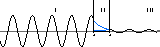
\includegraphics[width=0.9\textwidth]{Abb/tunnel.pdf}
   \caption{Skizze des Tunneleffekts: Die Wellenfunktion des Teilchens läuft von 
            links auf die Potentialbarriere zu. Nach einem exponentiellen Abfall
            im Inneren der Barriere besteht eine kleine Wahrscheinlichkeit, dass
            sich das Teilchen rechts der Barriere aufhält}
   \label{tunnel} 
\end{figure}
Benutzt man die stationäre Schrödingergleichung
\[
    - \frac{\hbar^2}{2m} \frac{d^2}{dx^2} \Phi(x) + V(x) \Phi(x)
    = E \Phi(x)    
\]
so findet sich für die Teilchenwellenfunktion
\[
    \Psi(x) = 
        \begin{cases}
            A \, e^{ikx} + B \, e^{-ikx}, \quad x<-a\\
            C \, e^{-\kappa x} + D \, e^{\kappa x} \quad -a < x < a\\
            F \, e^{ikx} + G \, e^{-ikx}, \quad x<-a
        \end{cases}
\]
mit den Wellenzahlen $k=\sqrt{2mE}/\hbar$ und $\kappa = \sqrt{2m(V_0-E)}/\hbar$.
Die Koeffizienten $A$ bis $G$ beschreiben hierbei die Amplituden der jeweiligen
Wellen. Für das Beispiel einer von links einfallenden Welle, beschreibt $A$ die
Amplitude der ursprünglichen Welle und $B$ die, der an der Schwelle reflektierten
Welle. $F$ und $G$ beschreiben die Amplituden nach der Barriere. Für eine von links
einfallende Welle ist $G=0$, da rechts keine Welle mehr reflektiert werden kann.
$C$ und $D$ beschreiben die Amplituden der 
Schwingungen innerhalb der Barriere. Da $\kappa$ eine reelle Zahl ist, beschreibt 
die Wellenfunktion innerhalb der Barriere allerdings lediglich einen exponentiellen
Abfall. $C$ ist also die Amplitude, die die Welle beim Auftreffen auf die Barriere
besitzt.
Dies ist in Abbildung \ref{tunnel} skizziert.
Benutzt man nun die Anschlussbedingungen
\begin{align*}
    &x=-a: \quad A \, e^{-ika} + B \, e^{ika} = C \, e^{\kappa a} 
        + D \, e^{-\kappa a}\\
    &x=a: \quad F \, e^{+ika} + G \, e^{-ika} = C \, e^{-\kappa a} 
        + D \, e^{+\kappa a}
\end{align*}
und die Normalisierungsbedingung
\[
    \int \Psi^* (x) \Phi (x) dx = 1
\]
so kann man Ausdrücke für die einzelnen Koeffizienten erhalten. Für ein von links 
einfallendes Teilchen, also $G=0$, errechnet sich die Transmissionsamplitude 
$S(E)$ zu
\[
    S(E) = \frac{F}{A} = \frac{e^{-2ika}}{\cosh(2\kappa a) + \frac{i \varepsilon}{2}
                               \sinh(2\kappa a)}
\]
Die Wahrscheinlichkeit einer Transmission, der Durchlässigkeitskoeffizient, 
errechnet sich dann zu
\[
    | S(E) |^2 = \frac{1}{1+(1+(\varepsilon^2/4)) \, \sinh^2(2\kappa a)}
\]
Mit $\varepsilon = \frac{\kappa}{k}-\frac{k}{\kappa}$.
Nimmt man nun eine sehr hohe und breite Barriere an, also $\kappa a >> 1$, so
kann $\sinh (2 \kappa a) \approx (1/2) e^{2\kappa a} >> 1$ genähert werden.
Aus dem resultierende Term kann nach einigen Umformungen, die hier nicht genauer
gezeigt werden sollen, der folgende handliche Term gewonnen werden:
\[
    | S(E) |^2 = \exp\left(-4 \sqrt{2m(V_0-E)} \, \frac{a}{\hbar}\right)
\]
Zusammenfassend besteht also für ein Teilchen mit $E<V_0$ eine endliche 
Durchgangswahrscheinlichkeit durch eine Potentialbarriere, die durch 
obigen Term beschrieben wird. \cite{schwabl}

        \subsubsection{Anwendung im Rastertunnelmikroskop}

Zur Abtastung kommt eine scharfe Metallspitze zum Einsatz, die im Abstand weniger
Angstrøm über eine leitfähige Probe positioniert wird. Durch eine angelegte 
Tunnelspannung $U_t$ werden die Fermi-Niveaus der Spitze $E_{F,S}$ und der Probe
$E_{F,P}$ gegeneinander verschoben, schematisch in Abbildung \ref{tunnelstm} 
dargestellt.
\begin{figure}
    \centering
    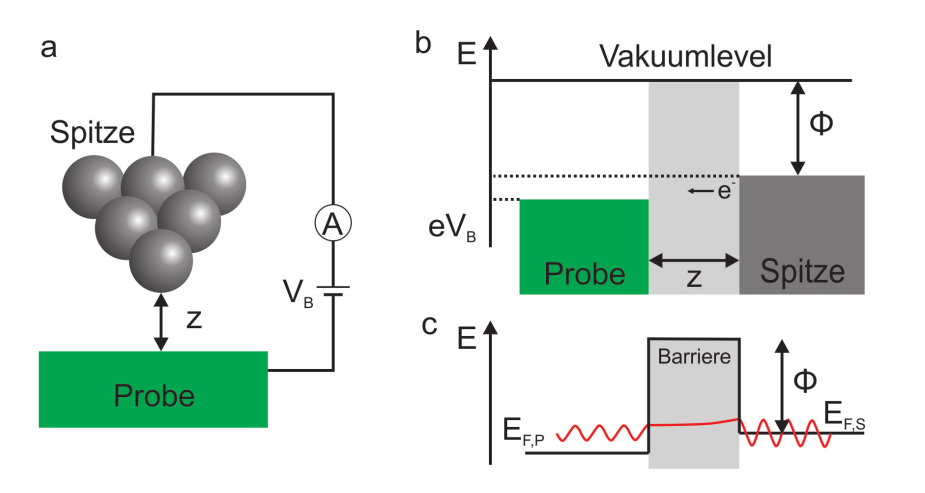
\includegraphics[width=0.8\textwidth]{Abb/tunnel_stm.png}
    \caption{a) Spitze und Probe werden über eine Spannungsquelle und einen 
                Strom-Spannungswandler miteinander verbunden. $V_B$ bezeichnet
                hier die Tunnelspannung, z den Abstand Spitze-Probe.
             b) Die angelegte Spannung verschiebt die beiden Fermi-Niveaus. Bei 
                positiver Spannung tunneln Elektronen der Spitze zur Probe.
             c) Tunneleffekt im STM.
             \cite{hofmann}}
    \label{tunnelstm}
\end{figure}
Der Strom $I_t$ zwischen Spitze und Probe ist nun von $U_t$ und dem Abstand $z$ 
abhängig. Das Abstandverhalten kann nun durch den eindimensionalen Tunnelprozess
hergeleitet werden. Die Höhe der Barriere ist die gemittelte Austrittsarbeit $\Phi$
des Spitzen- und Probenmaterials, also die nötige Energie Elektronen vom jeweiligen
Fermi-Niveau auf Vakuumenergie zu heben. Die Breite der Barriere ist der Abstand $z$.
Typischerweiße ist die angelegte Spannung sehr viel kleiner als $\Phi$, es kann also
eine rechteckige Barriere angenommen werden. Man erhält also:
\[
    I_t = I_0 \cdot e^{-2\kappa z}    
\]
$I_0$ gibt hierbei den Strom bei $z=0$, also den Strom bei Punktkontakt, 
an und $\kappa = \sqrt{2m \Phi}/ \hbar$ die Abklingkonstante, mit
der Elektronenmasse $m$. Für eine typische Austrittsarbeit $\Phi = \SI{5}{\eV}$
errechnet sich $\kappa = \SI{1}{\per \angstrom}$.\\
Für Metalle gilt näherungsweiße:
\[
    I_t \propto U_t \exp(-c_2 \sqrt{\Phi} z)
\]
mit $c_2 = \SI{1,025}{\per\angstrom\per\eV}$.
\cite{schwabl,hofmann}

\section{Aufbau eines Rastertunnelmikroskops}
\subsection{Herstellung der Spitze}

Eine STM-Spitze sollte sehr fein, dünn und starr sein, um die Messung selbst nicht zu verfälschen. Da das Bild einer STM-Messung durch die Faltung der Spitzenform mit der Form der gemessenen Oberfläche entsteht, sollte die Spitzenform möglichst nahe an einen Delta-Peak herankommen, um die Oberfläche optimal abbilden zu können. Zudem sollte die Spitze keine Oxidation aufweisen. Zur Herstellung wurden demnach zahlreiche Methoden entwickelt, wovon das für uns relevante Verfahren im Folgenden erläutert wird.


\subsubsection{Platin-Iridium Spitze}

\begin{figure}[h]
	\centering
	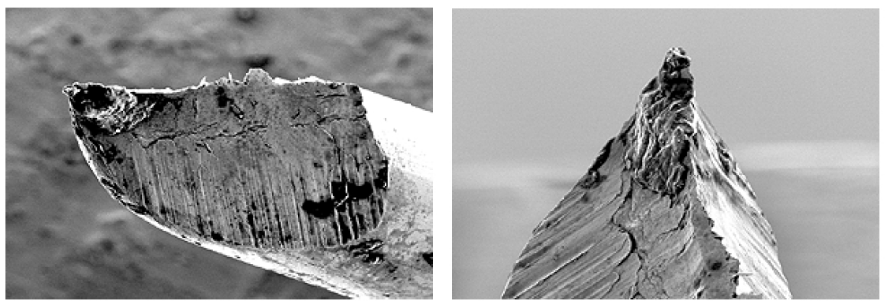
\includegraphics[width=0.7\textwidth]{Abb/pt-ir.png}
	\caption{Pt-Ir Spitze. \cite{nanosurf}}
	\label{ptir}
\end{figure}
Ein sehr einfaches Verfahren bietet die Platin-Iridium Spitze. Zur Herstellung wird
ein dünner Draht mit Zangen ruckartig abgerissen.\\
Die Vorgehensweiße ist in Abbildung \ref{ptirverf} dargestellt. Mit einer Flachzange
wird ein Ende des Drahtes festgehalten. Mit einem Seitenschneider wird unter sehr 
spitzem Winkel angesetzt, bis man Kontakt spürt. Dann wird mit dem Seitenschneider
ruckartig abgerissen.

Der große Vorteil dieses Verfahrens ist natürlich die Einfachheit der Herstellung.
Außerdem bietet das Material eine gute Langlebigkeit. Der große Nachteil ist die
Inhomogenität der Beschaffenheit der Spitzen. Durch das zufällige Abreißen 
unterscheidet sich natürlich jede Spitze. \cite{nanosurf}, \cite{beschr}
\begin{figure}[H]
	\centering
	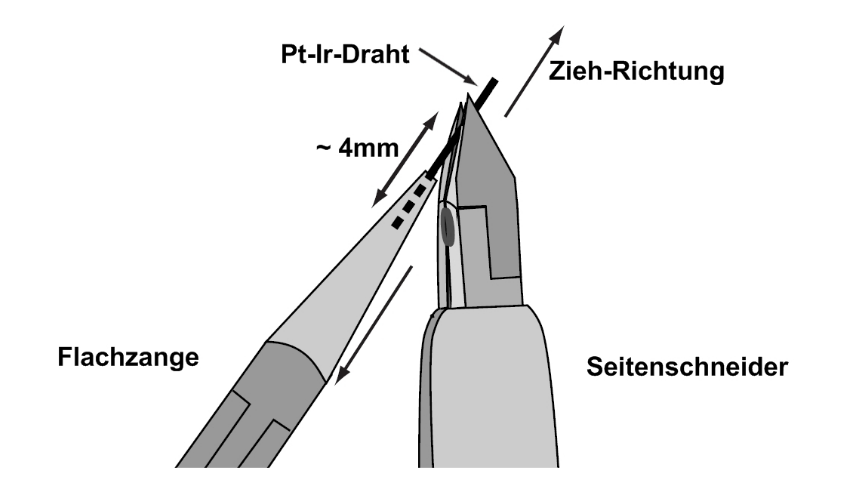
\includegraphics[width=0.6\textwidth]{Abb/pt-it-verf.png}
	\caption{Abreißen eines Platin-Iridiumdrahts. \cite{nanosurf}}
	\label{ptirverf}
\end{figure}

\subsection{Scanner-Einheit}


In Abbildung \ref{scan} ist der schematische Aufbau der Scanner-Einheit gezeigt.
Die leitende Spitze wird durch drei Piezos, pro Raumrichtung ein Piezoelement, 
über der Probe positioniert. Die Längenänderung der Kristalle ist annähernd linear
zur angelegten Spannung. Dies erlaubt eine einfache Steuerung des Aufbaus. Die 
Position kann nanometergenau verändert werden, die 
Piezomotoren übernehmen also die Feinannäherung der Spitze.
Die Erklärung des Piezoelektrischen Effekts erfolgt im nächsten Abschnitt.
\begin{figure}[H]
	\centering
	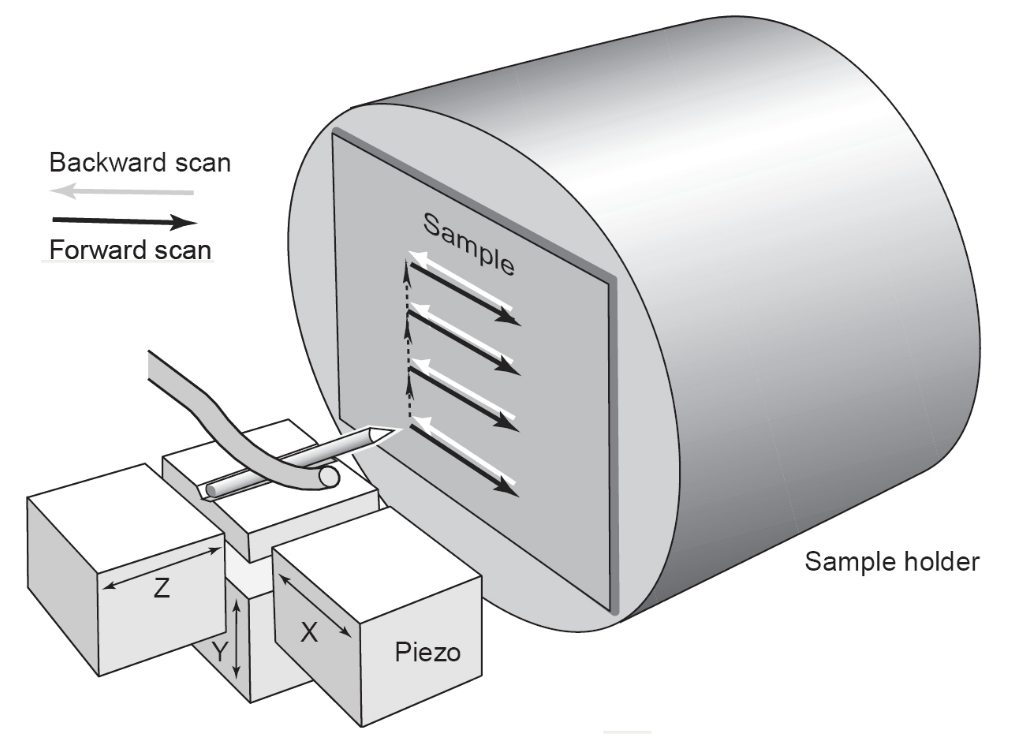
\includegraphics[width=0.6\textwidth]{Abb/scanner.png}
	\caption{Scanner-Einheit eines STM. \cite{nanosurf}}
	\label{scan}
\end{figure}


 \subsection{Piezoelektrischer Effekt}

\begin{wrapfigure}{r}{0.45\textwidth}
	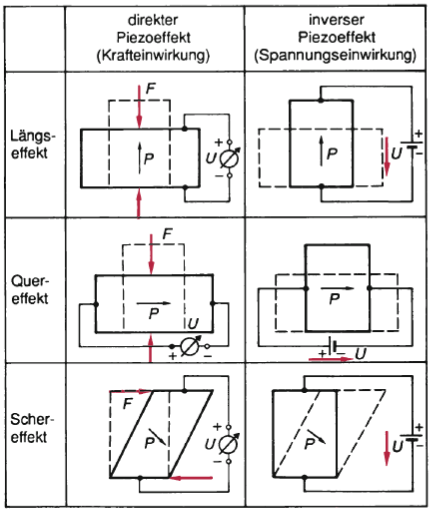
\includegraphics[width=0.45\textwidth]{Abb/piezo.png}
	\caption{Piezoelektrizität \cite{phying}}
	\label{piezo}
\end{wrapfigure}
Bestimmte Materialien erzeugen eine elektrische Spannung, sobald eine äußere Kraft
auf den Körper wirkt. Dies wird als piezoelektrischer Effekt bezeichnet. Er wurde
1880 durch die Brüder Curie an einigen Kristallen entdeckt.\\
Essentiell für die Rastersondenmikroskopie ist der inverse piezoelektrische Effekt.
Dieser führt zu einer Geometrieänderung des Kristalls beim Anlegen einer äußeren 
Spannung. Dies ermöglicht sehr feine Ortsänderungen der Spitze. Es werden drei 
technische nutzbare Vorgänge unterschieden, die in Abbildung \ref{piezo} skizziert
werden.
\begin{itemize}
	\item Längs-Effekt:\\
	Eine äußere Kraft $\textbf{F}$ führt zu einer Polarisierung $\textbf{P}$.
	Die resultierende Spannung $U$ liegt in gleicher Richtung an.
	\item Quer-Effekt:\\
	Eine äußere Kraft $\textbf{F}$ führt zu einer transversalen Polarisation
	$\textbf{P}$. Die resultierende Spannung $U$ liegt nun quer an.
	\item Scher-Effekt:\\
	Eine äußere Kraft $\textbf{F}$ führt zu einer diagonalen Polarisation
	$\textbf{P}$. Die resultierende Spannung $U$ liegt wiederum quer an.
\end{itemize} 
Der Piezoelektrische Effekt bietet somit also eine hervorragende Möglichkeit z.B. eine Spitze im STM durch Anlegen einer Spannung sehr präzise zu steuern. Die angelegte Spannung bewegt sich hierbei normalerweise in der Größenordnung von etwa $100\si{\volt}$.
\cite{phying} 

        

\section{Betriebsarten eines Rastertunnelmikroskops}
	\subsection{Rastern}
	Wie der Name des Rastertunnelmikroskops nahe legt, werden die Proben beim Mikroskopieren abgerastert. Das bedeutet, dass die Spitze solange in nahe beieinander liegenden parallelen Bahnen über den Messbereich fährt, bis dieser komplett erfasst wurde.
    \subsection{Topographischer Modus}
   

\begin{figure}[H]
    \centering
    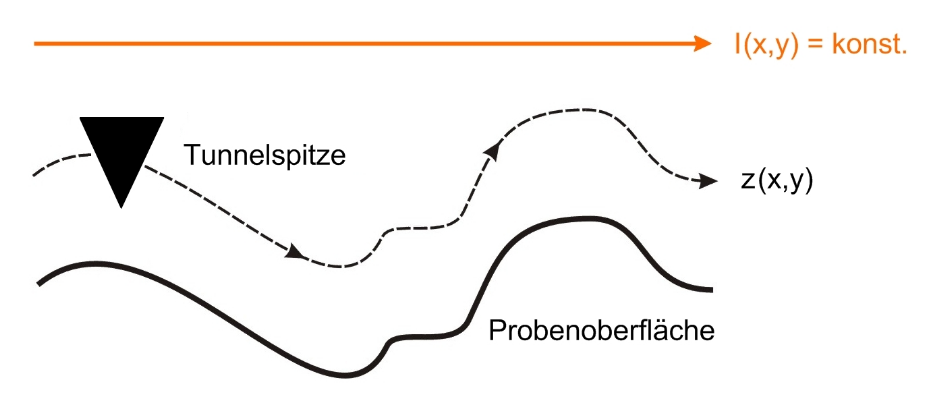
\includegraphics[width=0.8\textwidth]{Abb/topo.png}
    \caption{Topographischer Modus des STM. \cite{beschr}}
    \label{topo}
\end{figure}
Im topographischen Modus folgt die Spitze der Oberflächenbeschaffenheit der Probe,
wie in Abbildung \ref{topo} skizziert. Der Tunnelstrom soll durch Veränderung der 
z-Position beim Abrastern konstant gehalten werden. Das eigentliche Messsignal 
ist dann die Regelspannung des Piezoelements in z-Richtung. Der Nachteil dieser 
Messmethode ist die langsame Scangeschwindigkeit, die aus der ständigen 
Nachjustierung der z-Position resultiert.

    \subsection{Modus konstanter Höhe}

\begin{figure}[h]
    \centering
    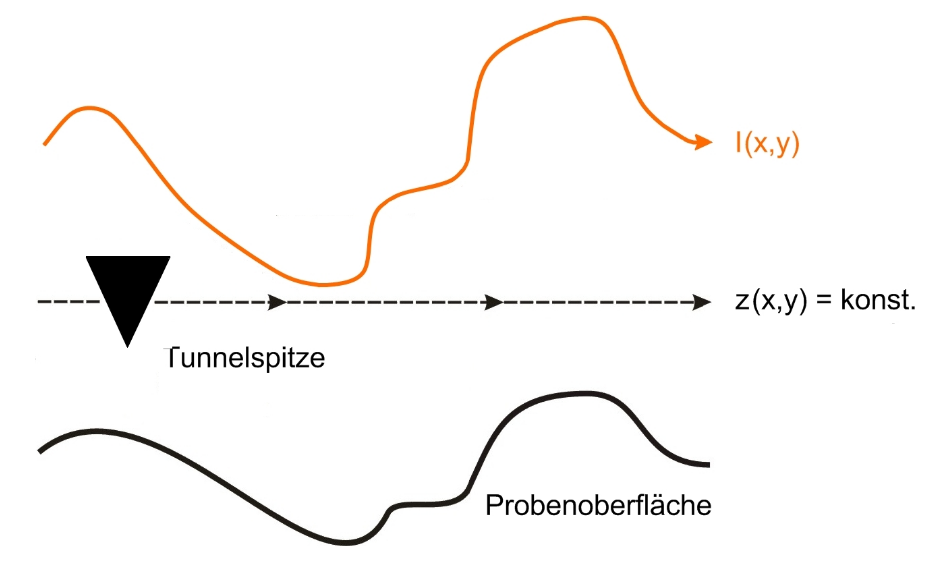
\includegraphics[width=0.7\textwidth]{Abb/konst.png}
    \caption{Modus konstanter Höhe des STM \cite{beschr}}
    \label{konst}
\end{figure}
In diesem Modus rastert die Spitze mit gleichbleibender z-Position, wie in Abbildung
\ref{konst} skizziert. So wird der
sich ändernde Tunnelstrom gemessen und daraus die Oberflächenbeschaffenheit der 
Probe rekonstruiert. Vorteil hierbei ist die hohe Scangeschwindigkeit. Nachteil
ist die Kollissionsgefahr, wodurch Spitze und Probe zerstört werden können. Dieser
Modus wird also nur bei vorheriger Kenntnis der Oberflächenstruktur eingesetzt, um 
nochmals genauere Messungen durchzuführen. Im Rahmen dieses Versuch wird 
ausschließlich der topographische Modus verwendet.

    \subsection{Spektroskopie}
    \label{spek}

Die Spektroskopie ermöglicht die Messung der lokalen Zustandsdichten (LDOS) der
Probe. Hierzu wird die Position der Spitze relativ zur Probe in allen Raumrichtungen
konstant gehalten. Zusätzlich zur Gleichspannung $U_t$ wird eine Wechselspannung an 
die Spitze angelegt. Unter Variation der Gleichspannung wird nun der Tunnelstrom
gemessen. Zur Auswertung wird der Strom $I_t$ nach der Spannung $U(x,y,U)$ 
aufgetragen. Es gilt:
\[
    I_t \propto \int_0^{eU} \rho_P (E_F - eU + \varepsilon) \; 
                            \rho_S (E_F + \varepsilon) \, d \varepsilon
\]
Dabei gibt $\rho_P$ die Zustandsdichte der Probe und $\rho_S$ die der Spitze an.
$E_F$ steht für die Fermi-Energie und $e$ für die Elementarladung.
Zur Messung von $\rho_P$ muss $\rho_S$ also bekannt sein. Mit $\rho_S$ konstant
ergibt sich:
\[
    \frac{dI}{dU} \propto \rho_P (E_F - eU - \varepsilon)
\]
Die Ableitung des Tunnelstroms nach der Spannung ist also proportional zur 
Zustandsdichten der Probe. Dies erlaubt also eine Messung der Zustandsdichte.
Der im Versuch verwendete Aufbau erlaubt zwei Arten der Spektroskopie. Entweder
wird, wie oben beschrieben, die Position der Spitze konstant gehalten und der 
Tunnelstrom gemessen, oder man ändert den Abstand zur Probe, indem der z-Piezo
angesteuert wird und misst dann den Tunnelstrom. Hier erwartet man einen 
exponentiellen Abfall des Tunnelstroms mit steigendem Abstand. Im Versuch wird
letztere Art der Spektroskopie verwendet.
\cite{beschr}

\section{Interpretation einer STM-Messung}

Die theoretischen Hintergründe des Mikroskops wurden soweit geklärt. Um aber 
erfolgreich mit diesem zu arbeiten ist es nötig zu wissen, wie die Ergebnisse
zu interpretieren sind. 

In Abbildung \ref{vorb-graphit} ist die Messung eines Graphit Gitters zu sehen. 
Der gemessene Tunnelstrom ist farblich kodiert, desto heller eine Stelle, desto
größer der Tunnelstrom. Der Kontrast wurde hierbei maximiert, der kleinste 
gemessene Wert ist also schwarz, der höchste weiß. Wichtig ist nun, dass hier
nicht die eigentliche Oberfläche des Festkörpers abgebildet ist, sondern die
lokalen Zustandsdichten der Elektronen. Oft ähneln sich Oberflächentopographie 
und Oberfläche, doch z.B. bei sehr guten Leitern kann durch die starke 
Delokalisierung der Elektronen keine atomare Auflösung erreicht werden. Was 
genau gemessen wird, muss also für jede Probe einzeln genau durchdacht werden.

\begin{figure}[H]
	\centering
	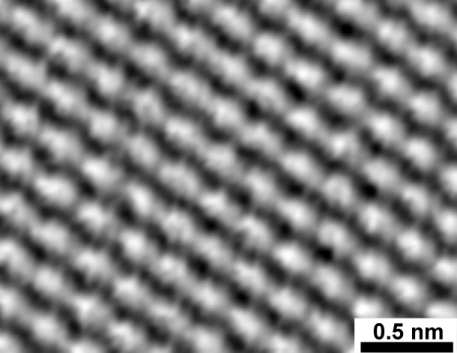
\includegraphics[width=0.5\textwidth]{Abb/graphit_messung.jpg}
	\caption{STM-Messung eines Graphit Gitters \cite{rasterwiki}}
	\label{vorb-graphit}
\end{figure}

\section{Probenmaterialien}
In diesem Versuch werden drei verschiedene Proben untersucht: Graphit, bzw. highly oriented pyrolytic graphite (HOPG), Gold (in der 111-Ebene) und Molybdänsulfid. Vor der Diskussion der Probenmaterialien sollen jedoch noch kurz die wichtigsten Gitterstrukturen von Festkörpern behandelt werden, welche auch in unseren Proben vorliegen.

\subsection{Kristallstrukturen im Festkörper}
\subsubsection{Kubische Gitter}


Es existieren drei verschiedene kubische Gitter.
Diese sind in Abbildung \ref{kub} dargestellt. Im Rahmen dieses Versuches
soll nur das kubisch flächenzentrierte Gitter näher betrachtet werden. Viele Metalle
und Legierungen kristallisieren in diese Anordnung.\\

\begin{figure}[H]
	\centering
	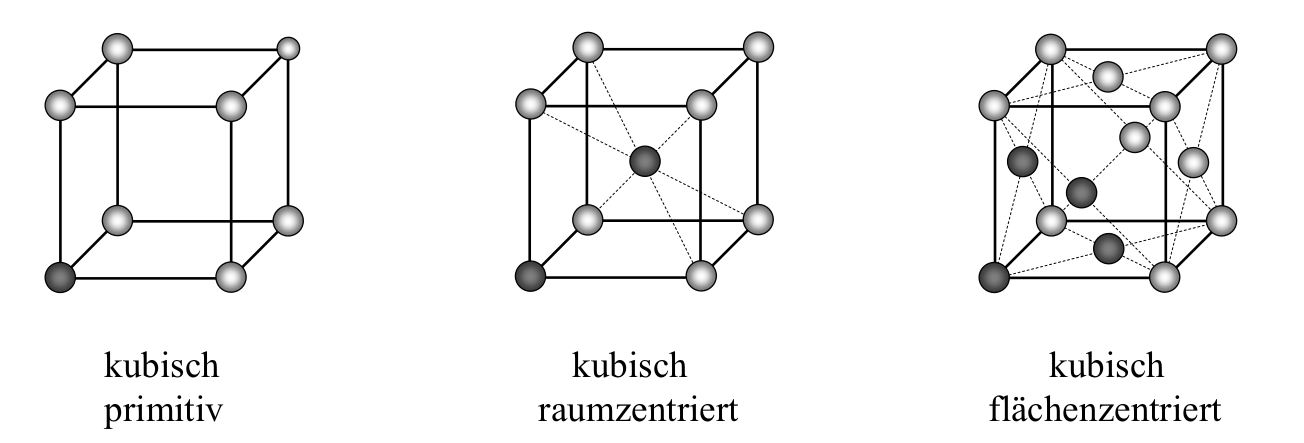
\includegraphics[width=0.9\textwidth]{Abb/kubische_gitter.png}
	\caption{Die drei kubischen Atomgitter. Von links nach rechts: 
		einfach kubisch (sc), kubisch raumzentriert (bcc),
		kubisch flächenzentriert (fcc) \cite{hunklinger}}
	\label{kub}
\end{figure}
\begin{figure}
	\centering
	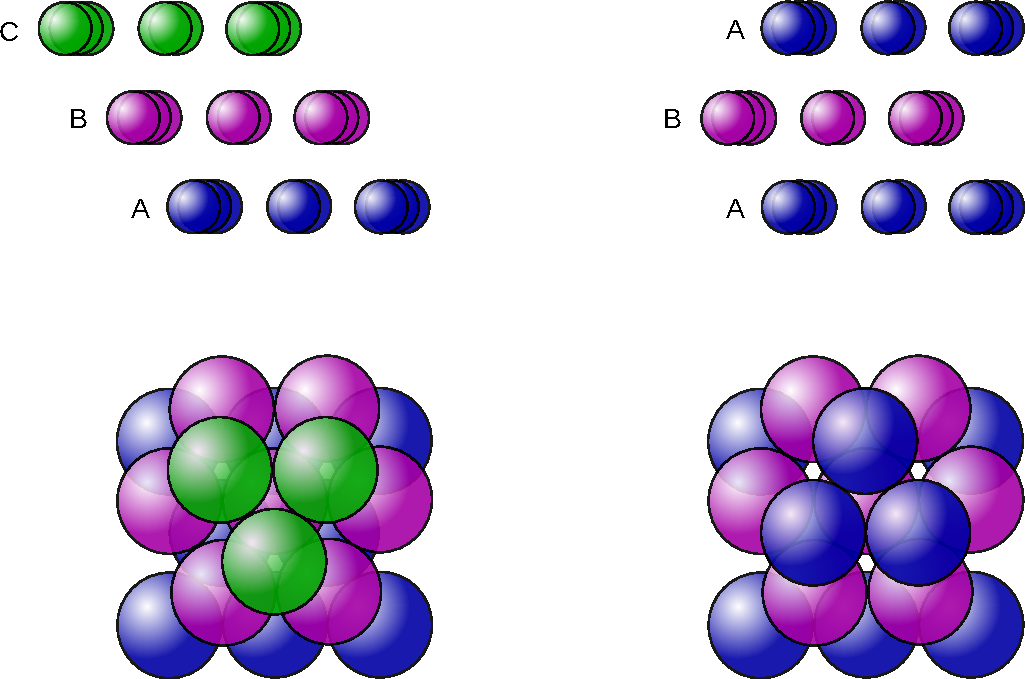
\includegraphics[width=0.7\textwidth]{Abb/DichtesteKugelpackung.pdf}
	\caption{Die möglichen Stapelfolgen für eine dichteste Kugelpackung:
		Links im Bild werden drei verschiedene Schichten gestapelt,
		also ABCABC... 
		Rechts werden nur zwei Schichten gestapelt, die dritte Schicht liegt
		also exakt auf der Ersten, ABABAB... \cite{kugel}}
	\label{pack}
\end{figure}
Betrachtet man eine möglichst dichte Packung an Kugeln, so sind zwei Stapelfolgen 
möglich. Das fcc-Gitter repräsentiert hierbei die Schichtfolge ABCABC..., siehe 
hierzu Abbildung \ref{pack}. Ein Atom hat in dieser Anordnung 12 nächste Nachbarn
mit dem Abstand $\frac{a}{\sqrt{2}}$. $a$ sei hier die Gitterkonstante des Würfels.
In einer kubischer Zelle befinden sich $8 \cdot \frac{1}{8} + 6 \cdot \frac{1}{2} 
= 4$ Atome. Die Atome an den Ecken befinden sich in acht Zellen gleichzeitig, jene 
an den Flächen in zwei. Sie werden deshalb anteilig hinzugerechnet.
Die Packungsdichte $ V_{\text{Atome}} / V_{\text{kub. Zelle}} $ ergibt sich somit zu:
\[
\underset{\text{Volumen eines Atoms}}{
	\underbrace{
		\frac{4}{3} \left( \frac{d_{NN}}{2} \right)^2 \pi}} \cdot
\underset{\text{Atome pro kubischer Zelle}}{4} 
/ \, 
\underset{\text{Volumen des Würfels}}{a^3} \approx 0.74
\]
Die dichtest mögliche Kugelpackung nimmt also $74\%$ des Raums ein.

\subsubsection{Hexagonal dichteste Kugelpackung}

\begin{wrapfigure}{r}{0.45\textwidth}
	\centering
	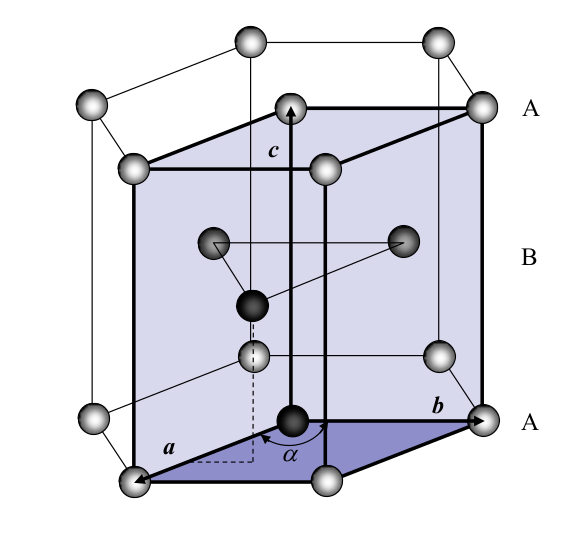
\includegraphics[width=0.4\textwidth]{Abb/hcp.png}
	\caption{hcp-Gitter \cite{hunklinger}}
	\label{hcp}
\end{wrapfigure}
Die rechte Stapelfolge in Abbildung \ref{pack} wird als hexagonal dichteste
Kugelpackung (hcp) bezeichnet. In Eigenschaften wie Abstand und Anzahl der nächsten
Nachbarn gleicht es dem fcc, was durch die Betrachtung als dichteste Packungen 
schnell klar wird. In Abbildung \ref{hcp} sind die Stapelfolgen eingezeichnet.
Die Vektoren $a$ und $b$ sind gleich lang. Für $c$ findet man $c = \sqrt{ 
	\frac{8}{3}} \, a$. In realen Kristallen weicht dies oft etwas ab.\par
\cite{hunklinger}

\subsection{HOPC}
Graphit besteht aus Schichten von in hexagonalem Muster angeordneten Kohlenstoffatomen (siehe Abb. \ref{hopc} ). Mit dem STM lässt sich diese Oberflächenstruktur jedoch nicht exakt wiedergeben, da bei je drei Atomen eines Sechsecks die Orbitale eine geringere Energie aufweisen. Elektronen können nun nicht mehr in diese Orbitale hineintunneln, wodurch sie für das STM "{}unsichtbar"{} werden. Dies ist in Abb. \ref{hopc}  dargestellt. Wir erwarten bei der Mikroskopie mit "{}atomarer"{} Auflösung also ein Muster aus gleichseitigen Dreiecken, insbesondere einen $60^\circ$-Winkel zwischen den Atomreihen.

\begin{figure}[h]
	\centering
	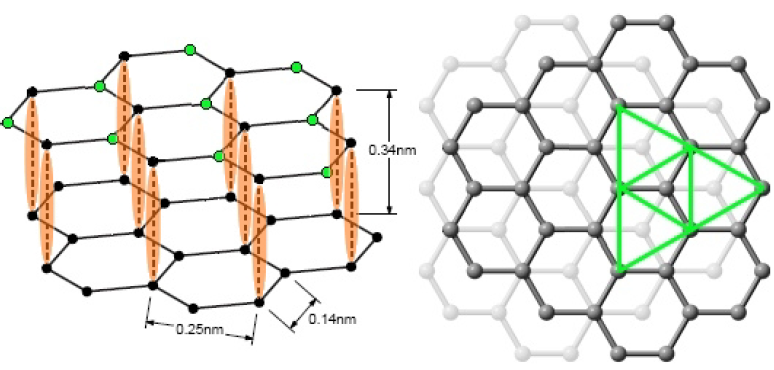
\includegraphics[width=\linewidth]{Mess/HOPC.png}
        \caption{Veranschaulichung der Verschiebung der Orbitale im HOPC. Atome der obersten Schicht, die direkt über Atomen der darunterliegenden Schicht sitzen, sind für das STM unsichtbar. Übrig und somit sichtbar bleiben nur Atome, die oberhalb eines Lochs der unteren Schicht liegen. Diese sind in der Abbildung grün dargestellt. \cite{beschr}}
	\label{hopc}
\end{figure}

\subsection{Gold}
Gold besitzt eine kubisch-flächenzentrierte Gitterstruktur (fcc), wovon wir im Versuch die 111-Ebene betrachten, siehe Abb.\ref{gold_struktur}. Da Gold eine sehr gleichmäßige Verteilung der Elektronen an der Oberfläche besitzt ("{}Elektronenwolke"), bleibt diese Struktur jedoch für das STM verborgen und wir müssen uns auf die Bestimmung der Stufenhöhe, also den Abstand zweier Schichten beschränken. Dieser liegt bei $0,236\si{\nano\meter}$.

\begin{figure}[h]
	\centering
	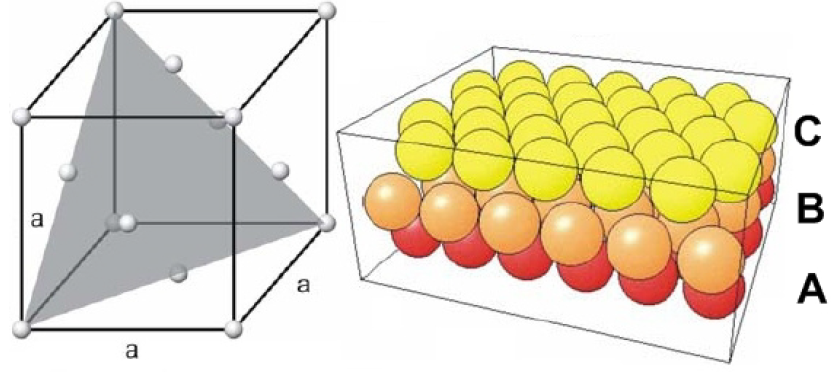
\includegraphics[width=\linewidth]{Mess/gold_struktur.png}
        \caption{Links: Darstellung der fcc-Gitters mit eingezeichneter 111-Ebene. Rechts: Anordnung der Atome in der 111-Ebene. \cite{beschr}}
	\label{gold_struktur}
\end{figure}

\subsection{Molybdänsulfid}
Zuletzt wird die Molybdänsulfidprobe gemessen. Hierbei handelt es sich um einen Halbleiter, der aus Schichten besteht, welche eine hexagonal dichteste Kugelpackung bilden (siehe Abb.\ref{mos_struktur}) und an dessen Oberfläche sich ausschließlich Schwefelatome befinden. Der Abstand der Schwefelatome beträgt $3,16\si{\angstrom}$. Theoretisch kann bei $\text{MoS}_{2}$ atomare Auflösung erreicht werden, jedoch gestaltet sich die Mikroskopie aufgrund des höheren Widerstands der Probe allgemein schwieriger.
\cite{beschr}

\begin{figure}[h]
	\centering
	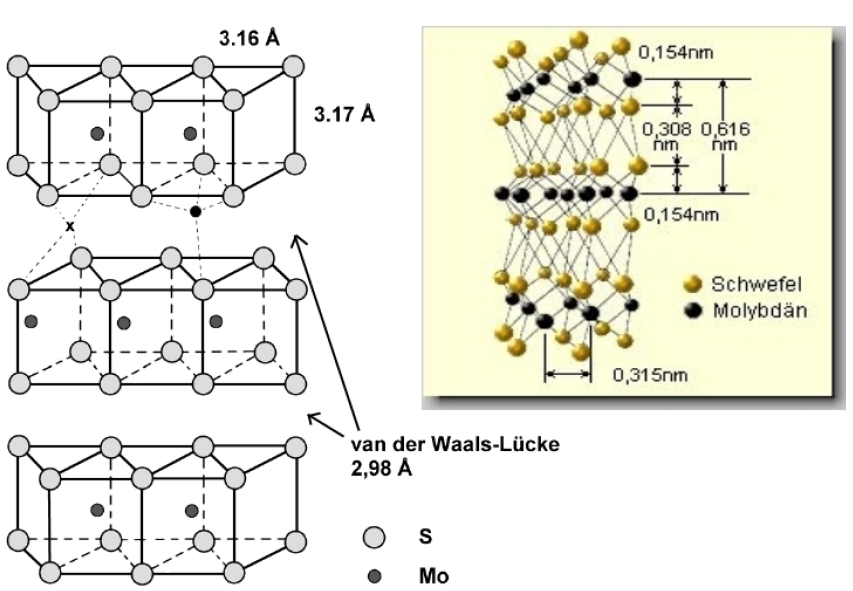
\includegraphics[width=\linewidth]{Mess/mos_struktur}
        \caption{Schematischer Aufbau der Molybdänsulfidprobe. Die einzelnen Schichten werden nur durch Van-der-Waals-Kräfte zusammengehalten. \cite{beschr}}
	\label{mos_struktur}
\end{figure}

